\let\negmedspace\undefined
\let\negthickspace\undefined
\documentclass[journal]{IEEEtran}
\usepackage[a5paper, margin=10mm, onecolumn]{geometry}
%\usepackage{lmodern} % Ensure lmodern is loaded for pdflatex
\usepackage{tfrupee} % Include tfrupee package

\setlength{\headheight}{1cm} % Set the height of the header box
\setlength{\headsep}{0mm}     % Set the distance between the header box and the top of the text

\usepackage{gvv-book}
\usepackage{gvv}
\usepackage{cite}
\usepackage{amsmath,amssymb,amsfonts,amsthm}
\usepackage{algorithmic}
\usepackage{graphicx}
\usepackage{textcomp}
\usepackage{xcolor}
\usepackage{txfonts}
\usepackage{listings}
\usepackage{enumitem}
\usepackage{mathtools}
\usepackage{gensymb}
\usepackage{comment}
\usepackage[breaklinks=true]{hyperref}
\usepackage{tkz-euclide} 
% \usepackage{gvv}                                        
\def\inputGnumericTable{}                                 
\usepackage[latin1]{inputenc}                                
\usepackage{color}                                            
\usepackage{array}                                            
\usepackage{longtable}                                       
\usepackage{calc}                                             
\usepackage{multirow}                                         
\usepackage{hhline}                                           
\usepackage{ifthen}                                           
\usepackage{lscape}
\begin{document}

\bibliographystyle{IEEEtran}
\vspace{3cm}

\title{8.EX-10}
\author{EE24BTECH11029 - J SHRETHAN REDDY}
\maketitle
% \newpage
% \bigskip
{\let\newpage\relax\maketitle}

\renewcommand{\thefigure}{\theenumi}
\renewcommand{\thetable}{\theenumi}
\setlength{\intextsep}{10pt} % Space between text and floats


\numberwithin{equation}{enumi}
\numberwithin{figure}{enumi}
\renewcommand{\thetable}{\theenumi}
\textbf{Question}:\\
Find the area of the region enclosed between the two circles: $x^2 + y^2 = 4$ and $\brak{x-2}^2 + y^2 = 4$\\
\textbf{Answer}:\\
\textbf{THEORETICAL SOLUTION}
\begin{align}
    x^2 + y^2 &= 4\\
    \brak{x-2}^2 +y^2 &=4
\end{align}
equate equation $\brak{0.1}$ and $\brak{0.2}$.we get
\begin{align}
    x = 1 \quad y = \pm\sqrt{3} 
\end{align}
The points of intersection of given circles are $A\brak{1,\sqrt{3}}$ and $A^{\prime}\brak{1,-\sqrt{3}}$ \\
Area of enclosed by two circles
\begin{align}
    area &= 2\sbrak{\int_0^1 y\,dx +\int_1^2 y\,dx}\\
         &=2\sbrak{\int_0^1 \sqrt{4-\brak{x-2}^2}\,dx +\int_1^2 \sqrt{4-x^2}\,dx}\\
         &=2\left[ \frac{1}{2}\brak{x-2}\sqrt{4-\brak{x-2}^2}+\frac{1}{2}\times4\sin^{-1}\frac{x-2}{2}\right]_0^1 + 2\left[ \frac{1}{2}x\sqrt{4-x^2}+\frac{1}{2}\times4\sin^{-1}\frac{x}{2}\right]_1^2\\
         &=\left[\brak{-\sqrt{3}-4\sin^{-1}}\brak{\frac{-1}{2}}-4\sin^{-1}\brak{-1}\right] + \left[4\sin^{-1}1-\sqrt{3}-4\sin^{-1}\frac{1}{2}\right]\\
         &=\brak{-\sqrt{3}-\frac{2\pi}{3}+2\pi}+\brak{2\pi-\sqrt{3}-\frac{2\pi}{3}}\\
         &=\frac{8\pi}{3}-2\sqrt{3}
\end{align}
\textbf{Computational Solution:}\\
Using the trapezoidal rule to get the area\\
The trapezoidal rule is as follows.\\
\begin{align}
    A &= \int_a^b f\brak{x}\,dx\approx h\brak{\frac{1}{2}f\brak{a}+f\brak{x_1}+f\brak{x_2}\dots+f\brak{x_{n-1}}+\frac{1}{2}f\brak{b}}\\
    h&=\frac{b-a}{n}\\
    A &= j_n,\quad where ,\quad j_{i+1}=j_i +h\frac{f\brak{x_{i+1}}+f\brak{x_i}}{2}\\
    j_{i+1}&= j_i+h\brak{\sqrt{x_{i+1}}+\sqrt{x_i}}\\
    x_{i+1}&=x_i +h\\
    h&=\frac{1}{30000}\\
    n&=30000
\end{align}
Using the code answer obtained is $A=1.369707sq$.units 
\begin{figure}[h!]
    \centering
    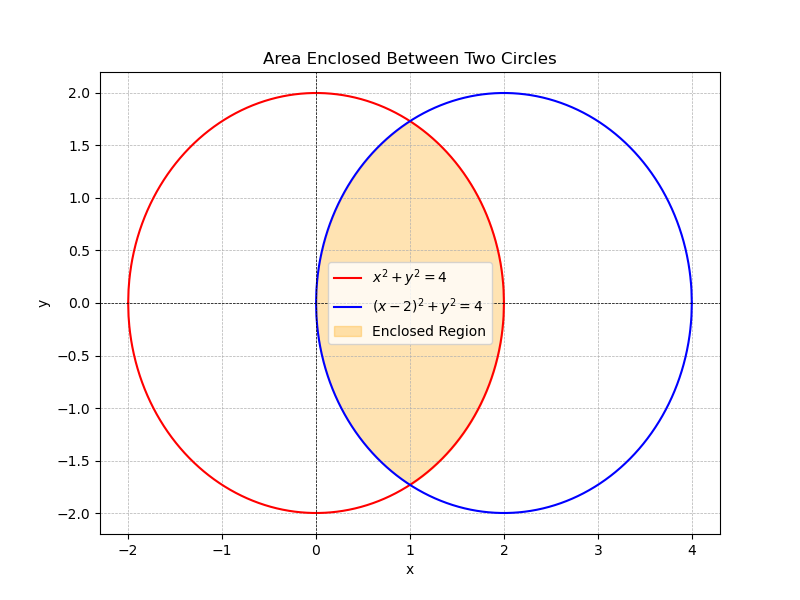
\includegraphics[width=1\columnwidth]{figure/fig.png} 
    \caption{plot}
    \label{stemplot}
 \end{figure}



\end{document}
